% Options for packages loaded elsewhere
\PassOptionsToPackage{unicode}{hyperref}
\PassOptionsToPackage{hyphens}{url}
\documentclass[
  spanish,
]{article}
\usepackage{xcolor}
\usepackage[margin=1in]{geometry}
\usepackage{amsmath,amssymb}
\setcounter{secnumdepth}{5}
\usepackage{iftex}
\ifPDFTeX
  \usepackage[T1]{fontenc}
  \usepackage[utf8]{inputenc}
  \usepackage{textcomp} % provide euro and other symbols
\else % if luatex or xetex
  \usepackage{unicode-math} % this also loads fontspec
  \defaultfontfeatures{Scale=MatchLowercase}
  \defaultfontfeatures[\rmfamily]{Ligatures=TeX,Scale=1}
\fi
\usepackage{lmodern}
\ifPDFTeX\else
  % xetex/luatex font selection
\fi
% Use upquote if available, for straight quotes in verbatim environments
\IfFileExists{upquote.sty}{\usepackage{upquote}}{}
\IfFileExists{microtype.sty}{% use microtype if available
  \usepackage[]{microtype}
  \UseMicrotypeSet[protrusion]{basicmath} % disable protrusion for tt fonts
}{}
\makeatletter
\@ifundefined{KOMAClassName}{% if non-KOMA class
  \IfFileExists{parskip.sty}{%
    \usepackage{parskip}
  }{% else
    \setlength{\parindent}{0pt}
    \setlength{\parskip}{6pt plus 2pt minus 1pt}}
}{% if KOMA class
  \KOMAoptions{parskip=half}}
\makeatother
\usepackage{graphicx}
\makeatletter
\newsavebox\pandoc@box
\newcommand*\pandocbounded[1]{% scales image to fit in text height/width
  \sbox\pandoc@box{#1}%
  \Gscale@div\@tempa{\textheight}{\dimexpr\ht\pandoc@box+\dp\pandoc@box\relax}%
  \Gscale@div\@tempb{\linewidth}{\wd\pandoc@box}%
  \ifdim\@tempb\p@<\@tempa\p@\let\@tempa\@tempb\fi% select the smaller of both
  \ifdim\@tempa\p@<\p@\scalebox{\@tempa}{\usebox\pandoc@box}%
  \else\usebox{\pandoc@box}%
  \fi%
}
% Set default figure placement to htbp
\def\fps@figure{htbp}
\makeatother
\ifLuaTeX
\usepackage[bidi=basic]{babel}
\else
\usepackage[bidi=default]{babel}
\fi
% get rid of language-specific shorthands (see #6817):
\let\LanguageShortHands\languageshorthands
\def\languageshorthands#1{}
\setlength{\emergencystretch}{3em} % prevent overfull lines
\providecommand{\tightlist}{%
  \setlength{\itemsep}{0pt}\setlength{\parskip}{0pt}}
\usepackage{booktabs}
\usepackage{longtable}
\usepackage{array}
\usepackage{multirow}
\usepackage{float}
\usepackage{colortbl}
\usepackage{xcolor}
\usepackage{pdflscape}
\usepackage{geometry}
\geometry{margin=2.5cm}
\usepackage{fancyhdr}
\pagestyle{fancy}
\fancyhead[L]{\small Descriptivos, Confiabilidad y Supuestos}
\fancyhead[R]{\small Tesis --- Experiencia Gastronómica}
\fancyfoot[C]{\thepage}
\renewcommand{\headrulewidth}{0.4pt}
\usepackage{caption}
\captionsetup{font=small, labelfont=bf}
\usepackage{booktabs}
\usepackage{longtable}
\usepackage{array}
\usepackage{multirow}
\usepackage{wrapfig}
\usepackage{float}
\usepackage{colortbl}
\usepackage{pdflscape}
\usepackage{tabu}
\usepackage{threeparttable}
\usepackage{threeparttablex}
\usepackage[normalem]{ulem}
\usepackage{makecell}
\usepackage{xcolor}
\usepackage{bookmark}
\IfFileExists{xurl.sty}{\usepackage{xurl}}{} % add URL line breaks if available
\urlstyle{same}
\hypersetup{
  pdftitle={Análisis Descriptivo, Confiabilidad y Verificación de Supuestos},
  pdfauthor={Martín Vargas Estrada},
  pdflang={es},
  hidelinks,
  pdfcreator={LaTeX via pandoc}}

\title{Análisis Descriptivo, Confiabilidad y Verificación de Supuestos}
\usepackage{etoolbox}
\makeatletter
\providecommand{\subtitle}[1]{% add subtitle to \maketitle
  \apptocmd{\@title}{\par {\large #1 \par}}{}{}
}
\makeatother
\subtitle{Impacto de los factores de la experiencia gastronómica en la
toma de decisiones del comensal}
\author{Martín Vargas Estrada}
\date{08 de Marzo de 2026}

\begin{document}
\maketitle

{
\setcounter{tocdepth}{3}
\tableofcontents
}
\section{Carga de datos y
librerías}\label{carga-de-datos-y-libreruxedas}

Se trabaja con el data frame \texttt{datos} generado en el informe de
preparación (176 observaciones: 44 comensales \(\times\) 4 condiciones
experimentales).

\section{Estadísticos descriptivos}\label{estaduxedsticos-descriptivos}

\subsection{Descriptivos globales por
ítem}\label{descriptivos-globales-por-uxedtem}

\begin{table}[!h]
\centering
\begin{tabular}{lccc}
\toprule
Ítem & Media & DE & Mediana\\
\midrule
\addlinespace[0.3em]
\multicolumn{4}{l}{\textbf{Producto}}\\
\hspace{1em}P1 & 3.05 & 0.97 & 3\\
\hspace{1em}P2 & 3.42 & 0.95 & 3\\
\hspace{1em}P3 & 3.34 & 1.05 & 3\\
\addlinespace[0.3em]
\multicolumn{4}{l}{\textbf{Servicio}}\\
\hspace{1em}S1 & 3.82 & 1.11 & 4\\
\hspace{1em}S2 & 3.81 & 1.09 & 4\\
\hspace{1em}S3 & 4.13 & 0.91 & 4\\
\addlinespace[0.3em]
\multicolumn{4}{l}{\textbf{Entorno}}\\
\hspace{1em}E1 & 3.94 & 1.21 & 4\\
\hspace{1em}E2 & 3.87 & 1.19 & 4\\
\hspace{1em}E3 & 3.49 & 1.04 & 4\\
\hspace{1em}E4 & 3.71 & 1.00 & 4\\
\hspace{1em}E5 & 3.98 & 0.93 & 4\\
\hspace{1em}E6 & 3.76 & 1.44 & 4\\
\hspace{1em}E7 & 3.65 & 1.46 & 4\\
\hspace{1em}E8 & 3.38 & 1.51 & 4\\
\addlinespace[0.3em]
\multicolumn{4}{l}{\textbf{Variables dependientes}}\\
\hspace{1em}I1 & 3.24 & 0.98 & 3\\
\hspace{1em}I2 & 3.08 & 1.03 & 3\\
\bottomrule
\end{tabular}
\end{table}

\subsection{Descriptivos por condición
experimental}\label{descriptivos-por-condiciuxf3n-experimental}

\begin{landscape}
\begin{table}[!h]
\centering\begingroup\fontsize{10}{12}\selectfont

\begin{tabular}{lccccccccccc}
\toprule
\multicolumn{1}{c}{ } & \multicolumn{2}{c}{Producto} & \multicolumn{2}{c}{Servicio} & \multicolumn{2}{c}{Entorno} & \multicolumn{2}{c}{Satisfacción} & \multicolumn{2}{c}{Revisitar} & \multicolumn{1}{c}{Recom.} \\
\cmidrule(l{3pt}r{3pt}){2-3} \cmidrule(l{3pt}r{3pt}){4-5} \cmidrule(l{3pt}r{3pt}){6-7} \cmidrule(l{3pt}r{3pt}){8-9} \cmidrule(l{3pt}r{3pt}){10-11} \cmidrule(l{3pt}r{3pt}){12-12}
Condición & M & DE & M & DE & M & DE & M & DE & M & DE & \%\\
\midrule
Base (todo bien) & 3.77 & 0.57 & 4.30 & 0.62 & 4.33 & 0.39 & 4.07 & 0.45 & 4.09 & 0.64 & 95.5\\
Servicio degradado & 3.44 & 0.72 & 3.11 & 1.02 & 4.11 & 0.56 & 3.23 & 0.91 & 3.02 & 0.98 & 47.7\\
Producto degradado & 2.72 & 0.63 & 4.33 & 0.66 & 4.16 & 0.43 & 2.86 & 0.98 & 2.61 & 0.81 & 29.5\\
Entorno degradado & 3.15 & 0.93 & 3.95 & 0.84 & 2.29 & 0.73 & 2.82 & 0.92 & 2.59 & 0.90 & 29.5\\
\bottomrule
\end{tabular}
\endgroup{}
\end{table}
\end{landscape}

\subsection{Distribución de las variables
dependientes}\label{distribuciuxf3n-de-las-variables-dependientes}

\begin{figure}[H]

{\centering 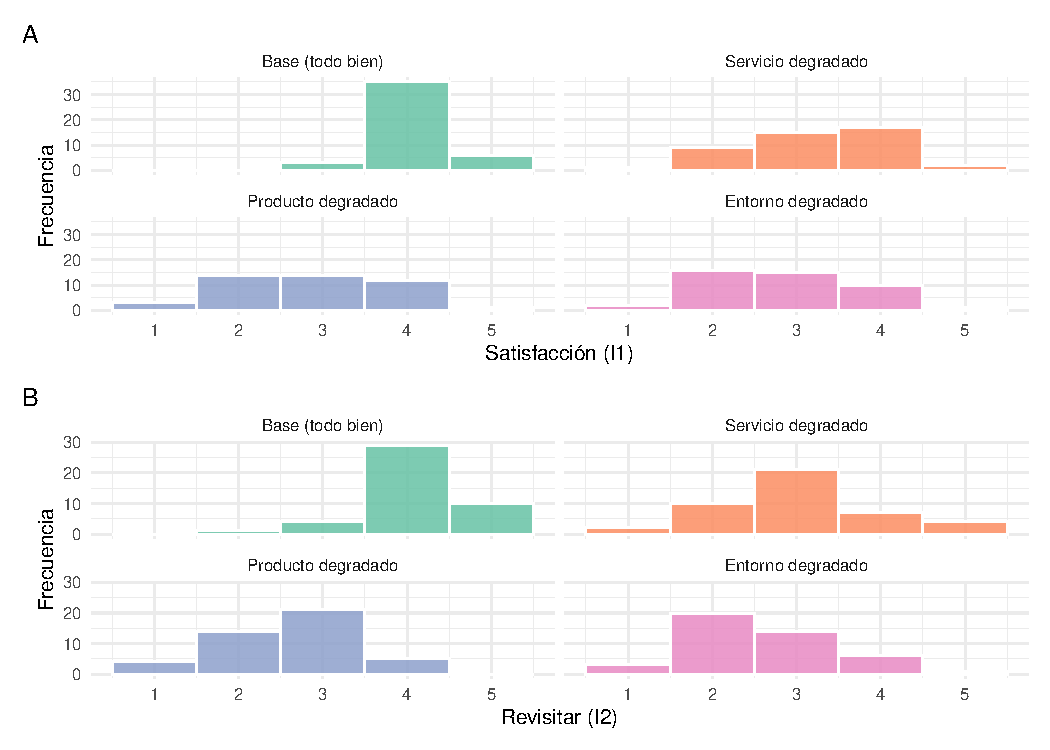
\includegraphics[width=0.95\linewidth]{01_descriptivos_confiabilidad_supuestos-1-_files/figure-latex/histogramas-vd-1} 

}

\caption{Distribución de las variables dependientes por condición experimental.}\label{fig:histogramas-vd}
\end{figure}

\begin{figure}[H]

{\centering 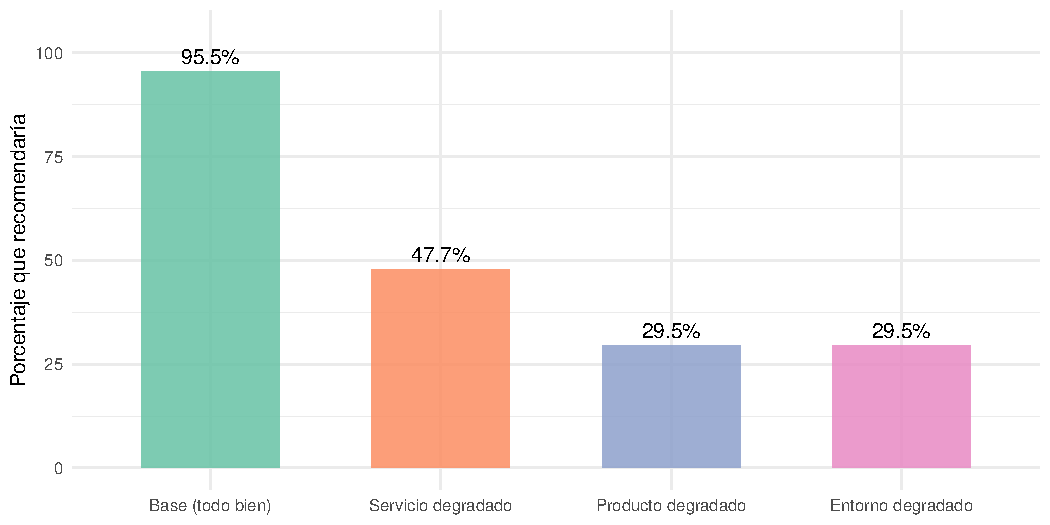
\includegraphics[width=0.95\linewidth]{01_descriptivos_confiabilidad_supuestos-1-_files/figure-latex/barras-recomendar-1} 

}

\caption{Proporción de comensales que recomendarían el establecimiento, por condición.}\label{fig:barras-recomendar}
\end{figure}

\subsection{Distribución de los índices por
dimensión}\label{distribuciuxf3n-de-los-uxedndices-por-dimensiuxf3n}

\begin{figure}[H]

{\centering 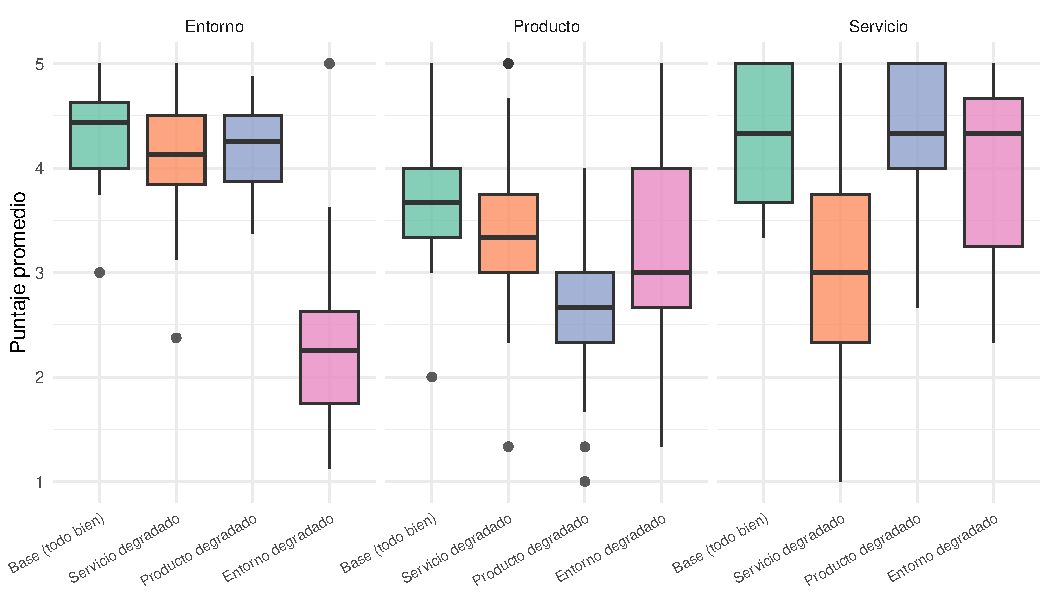
\includegraphics[width=0.95\linewidth]{01_descriptivos_confiabilidad_supuestos-1-_files/figure-latex/boxplots-dimensiones-1} 

}

\caption{Comparación de los índices de Producto, Servicio y Entorno por condición experimental.}\label{fig:boxplots-dimensiones}
\end{figure}

\newpage

\section{Análisis de confiabilidad (Alfa de
Cronbach)}\label{anuxe1lisis-de-confiabilidad-alfa-de-cronbach}

Se evalúa la consistencia interna de cada subescala para justificar el
uso de índices agregados. Se calcula el Alfa de Cronbach de forma global
(las 4 semanas juntas, \(n = 176\)) y por cada condición experimental
(\(n = 44\)).

\subsection{Confiabilidad global}\label{confiabilidad-global}

\begin{table}[!h]
\centering
\begin{tabular}{llc}
\toprule
Subescala & Ítems & $\alpha$\\
\midrule
Producto & P1, P2, P3 (3 ítems) & 0.768\\
Servicio & S1, S2, S3 (3 ítems) & 0.877\\
Entorno & E1--E8 (8 ítems) & 0.919\\
\bottomrule
\end{tabular}
\end{table}

Como referencia, valores de \(\alpha \geq 0.70\) se consideran
aceptables para investigación exploratoria, y \(\alpha \geq 0.80\) se
consideran buenos.

\subsection{Detalle ítem-total (contribución de cada
ítem)}\label{detalle-uxedtem-total-contribuciuxf3n-de-cada-uxedtem}

\subsubsection{Subescala Producto}\label{subescala-producto}

\begin{table}[!h]
\centering
\begin{tabular}{lccc}
\toprule
Ítem & $r_{ítem-total}$ & Media & DE\\
\midrule
P1 & 0.650 & 3.045 & 0.973\\
P2 & 0.568 & 3.420 & 0.947\\
P3 & 0.590 & 3.341 & 1.046\\
\bottomrule
\end{tabular}
\end{table}

\subsubsection{Subescala Servicio}\label{subescala-servicio}

\begin{table}[!h]
\centering
\begin{tabular}{lccc}
\toprule
Ítem & $r_{ítem-total}$ & Media & DE\\
\midrule
S1 & 0.807 & 3.824 & 1.115\\
S2 & 0.822 & 3.807 & 1.094\\
S3 & 0.682 & 4.131 & 0.913\\
\bottomrule
\end{tabular}
\end{table}

\subsubsection{Subescala Entorno}\label{subescala-entorno}

\begin{table}[!h]
\centering
\begin{tabular}{lccc}
\toprule
Ítem & $r_{ítem-total}$ & Media & DE\\
\midrule
E1 & 0.850 & 3.943 & 1.213\\
E2 & 0.807 & 3.869 & 1.186\\
E3 & 0.666 & 3.494 & 1.036\\
E4 & 0.540 & 3.710 & 0.998\\
E5 & 0.619 & 3.977 & 0.932\\
\addlinespace
E6 & 0.856 & 3.761 & 1.438\\
E7 & 0.839 & 3.648 & 1.458\\
E8 & 0.715 & 3.375 & 1.507\\
\bottomrule
\end{tabular}
\end{table}

\subsubsection{Alfa si se elimina el
ítem}\label{alfa-si-se-elimina-el-uxedtem}

\begin{table}[!h]
\centering
\caption{\label{tab:alpha-drop-prod}Subescala Producto}
\centering
\begin{tabular}[t]{lc}
\toprule
Ítem eliminado & $\alpha$ resultante\\
\midrule
P1 & 0.634\\
P2 & 0.724\\
P3 & 0.704\\
\bottomrule
\end{tabular}
\end{table}

\begin{table}[!h]
\centering
\caption{\label{tab:alpha-drop-serv}Subescala Servicio}
\centering
\begin{tabular}[t]{lc}
\toprule
Ítem eliminado & $\alpha$ resultante\\
\midrule
S1 & 0.788\\
S2 & 0.771\\
S3 & 0.898\\
\bottomrule
\end{tabular}
\end{table}

\begin{table}[!h]
\centering
\caption{\label{tab:alpha-drop-ent}Subescala Entorno}
\centering
\begin{tabular}[t]{lc}
\toprule
Ítem eliminado & $\alpha$ resultante\\
\midrule
E1 & 0.899\\
E2 & 0.903\\
E3 & 0.914\\
E4 & 0.922\\
E5 & 0.918\\
\addlinespace
E6 & 0.898\\
E7 & 0.900\\
E8 & 0.912\\
\bottomrule
\end{tabular}
\end{table}

\subsection{Confiabilidad por condición
experimental}\label{confiabilidad-por-condiciuxf3n-experimental}

\begin{table}[!h]
\centering
\begin{tabular}{lccc}
\toprule
Condición & $\alpha$ Producto & $\alpha$ Servicio & $\alpha$ Entorno\\
\midrule
Base (todo bien) & 0.509 & 0.813 & 0.619\\
Servicio degradado & 0.713 & 0.901 & 0.781\\
Producto degradado & 0.704 & 0.827 & 0.716\\
Entorno degradado & 0.810 & 0.798 & 0.870\\
\bottomrule
\end{tabular}
\end{table}

Si algún valor queda por debajo de 0.70 en una condición particular,
puede deberse al tamaño muestral reducido (\(n = 44\)) y no
necesariamente indica un problema con la escala, siempre que el alfa
global sea aceptable.

\newpage

\section{Verificación de supuestos para pruebas
inferenciales}\label{verificaciuxf3n-de-supuestos-para-pruebas-inferenciales}

Dado que las variables dependientes son ordinales (Likert 1--5), se
verifican los supuestos de normalidad y homocedasticidad para decidir
entre pruebas paramétricas (ANOVA) y no paramétricas (Kruskal-Wallis).

\subsection{Prueba de normalidad
(Shapiro-Wilk)}\label{prueba-de-normalidad-shapiro-wilk}

Se aplica el test de Shapiro-Wilk a cada variable dependiente dentro de
cada condición experimental (\(n = 44\) por grupo). La hipótesis nula es
que los datos provienen de una distribución normal.

\begin{table}[!h]
\centering\begingroup\fontsize{9}{11}\selectfont

\begin{tabular}{llcc>{}c}
\toprule
Variable & Condición & $W$ & $p$ & Normal ($\alpha=0.05$)\\
\midrule
Satisfacción (I1) & Base (todo bien) & 0.6177 & 0.0000 & \textcolor{red}{No}\\
Satisfacción (I1) & Servicio degradado & 0.8836 & 0.0004 & \textcolor{red}{No}\\
Satisfacción (I1) & Producto degradado & 0.8962 & 0.0008 & \textcolor{red}{No}\\
Satisfacción (I1) & Entorno degradado & 0.8876 & 0.0005 & \textcolor{red}{No}\\
Revisitar (I2) & Base (todo bien) & 0.7547 & 0.0000 & \textcolor{red}{No}\\
\addlinespace
Revisitar (I2) & Servicio degradado & 0.8919 & 0.0006 & \textcolor{red}{No}\\
Revisitar (I2) & Producto degradado & 0.8608 & 0.0001 & \textcolor{red}{No}\\
Revisitar (I2) & Entorno degradado & 0.8726 & 0.0002 & \textcolor{red}{No}\\
Índice Producto & Base (todo bien) & 0.9521 & 0.0661 & \textcolor{teal}{Sí}\\
Índice Producto & Servicio degradado & 0.9624 & 0.1603 & \textcolor{teal}{Sí}\\
\addlinespace
Índice Producto & Producto degradado & 0.9533 & 0.0728 & \textcolor{teal}{Sí}\\
Índice Producto & Entorno degradado & 0.9698 & 0.2966 & \textcolor{teal}{Sí}\\
Índice Servicio & Base (todo bien) & 0.8514 & 0.0000 & \textcolor{red}{No}\\
Índice Servicio & Servicio degradado & 0.9752 & 0.4533 & \textcolor{teal}{Sí}\\
Índice Servicio & Producto degradado & 0.8691 & 0.0001 & \textcolor{red}{No}\\
\addlinespace
Índice Servicio & Entorno degradado & 0.9006 & 0.0011 & \textcolor{red}{No}\\
Índice Entorno & Base (todo bien) & 0.9318 & 0.0121 & \textcolor{red}{No}\\
Índice Entorno & Servicio degradado & 0.9625 & 0.1614 & \textcolor{teal}{Sí}\\
Índice Entorno & Producto degradado & 0.9452 & 0.0366 & \textcolor{red}{No}\\
Índice Entorno & Entorno degradado & 0.9219 & 0.0055 & \textcolor{red}{No}\\
\bottomrule
\end{tabular}
\endgroup{}
\end{table}

\subsection{Gráficos Q-Q de las variables
dependientes}\label{gruxe1ficos-q-q-de-las-variables-dependientes}

\begin{figure}[H]

{\centering 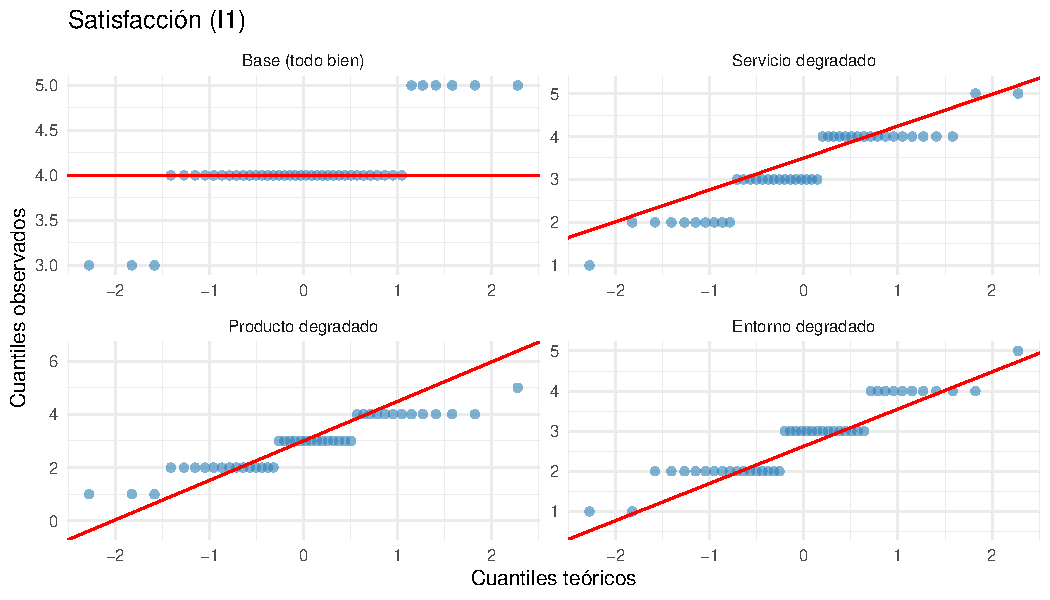
\includegraphics[width=0.95\linewidth]{01_descriptivos_confiabilidad_supuestos-1-_files/figure-latex/qq-satisfaccion-1} 

}

\caption{Gráficos Q-Q de Satisfacción (I1) por condición.}\label{fig:qq-satisfaccion}
\end{figure}

\begin{figure}[H]

{\centering 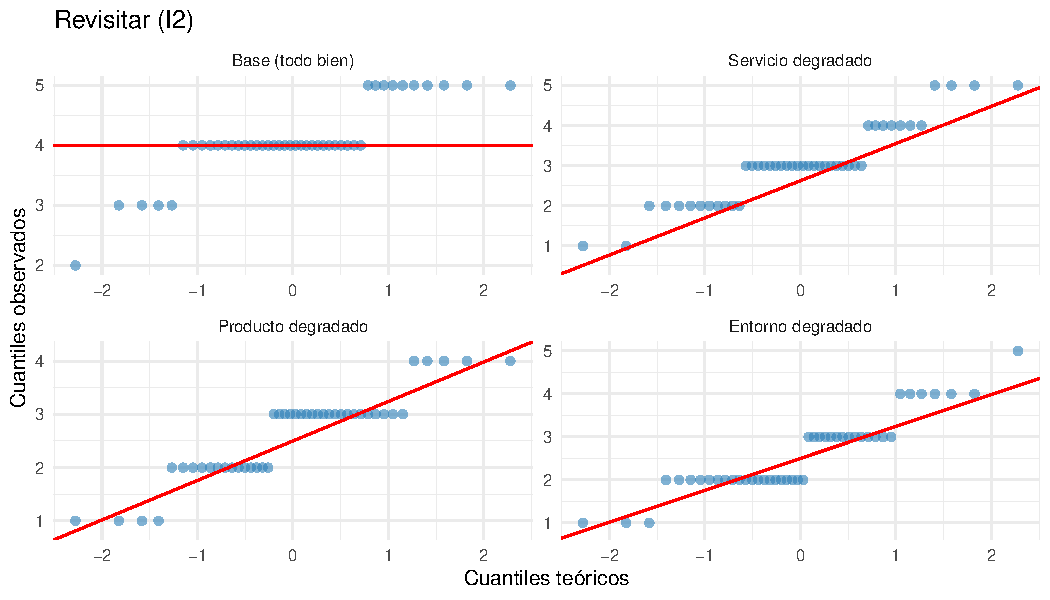
\includegraphics[width=0.95\linewidth]{01_descriptivos_confiabilidad_supuestos-1-_files/figure-latex/qq-revisitar-1} 

}

\caption{Gráficos Q-Q de Revisitar (I2) por condición.}\label{fig:qq-revisitar}
\end{figure}

\begin{figure}[H]

{\centering 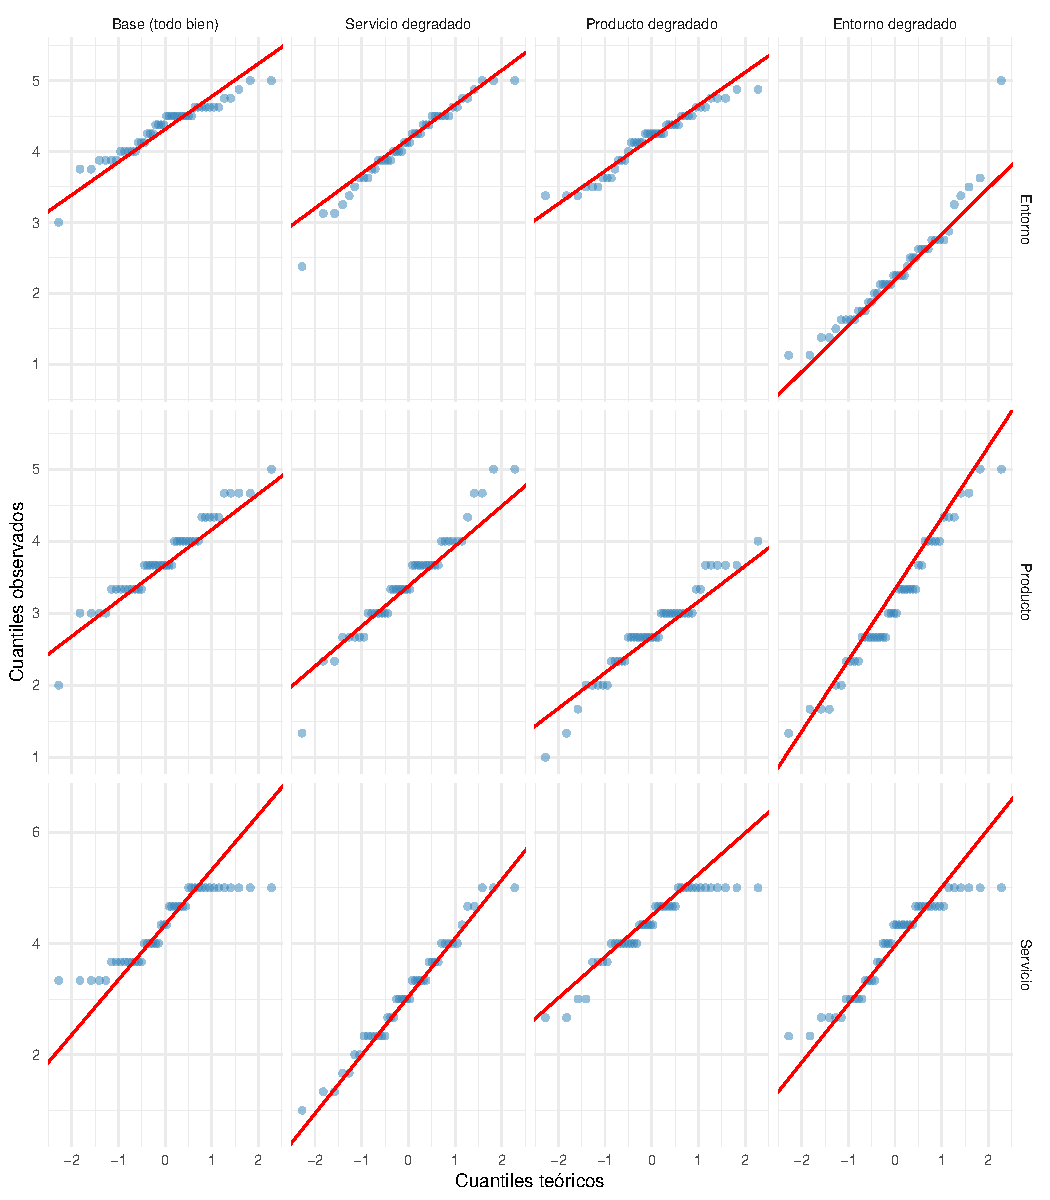
\includegraphics[width=0.95\linewidth]{01_descriptivos_confiabilidad_supuestos-1-_files/figure-latex/qq-indices-1} 

}

\caption{Gráficos Q-Q de los índices agregados (Producto, Servicio, Entorno) por condición.}\label{fig:qq-indices}
\end{figure}

\subsection{Prueba de homogeneidad de varianzas
(Levene)}\label{prueba-de-homogeneidad-de-varianzas-levene}

Se aplica el test de Levene (basado en la mediana, más robusto que el
basado en la media) para evaluar si las varianzas de cada variable
dependiente son homogéneas entre las cuatro condiciones. La hipótesis
nula es que las varianzas son iguales.

\begin{table}[!h]
\centering
\begin{tabular}{lcccc>{}c}
\toprule
Variable & $F$ & $gl_1$ & $gl_2$ & $p$ & Varianzas homogéneas\\
\midrule
Satisfacción (I1) & 10.524 & 3 & 172 & 0.0000 & \textcolor{red}{No}\\
Revisitar (I2) & 2.401 & 3 & 172 & 0.0695 & \textcolor{teal}{Sí}\\
Índice Producto & 4.398 & 3 & 172 & 0.0052 & \textcolor{red}{No}\\
Índice Servicio & 3.461 & 3 & 172 & 0.0176 & \textcolor{red}{No}\\
Índice Entorno & 3.586 & 3 & 172 & 0.0150 & \textcolor{red}{No}\\
\bottomrule
\end{tabular}
\end{table}

\newpage

\section{Resumen y decisión sobre pruebas a
utilizar}\label{resumen-y-decisiuxf3n-sobre-pruebas-a-utilizar}

\begin{table}[!h]
\centering\begingroup\fontsize{9}{11}\selectfont

\begin{tabular}{lll>{}l}
\toprule
Variable & Normalidad & Homocedasticidad & Prueba recomendada\\
\midrule
Revisitar (I2) & No cumple en 4 de 4 grupos & Cumple (Levene $p > .05$) & \textbf{Kruskal-Wallis + Dunn}\\
Satisfacción (I1) & No cumple en 4 de 4 grupos & No cumple (Levene $p \leq .05$) & \textbf{Kruskal-Wallis + Dunn}\\
Índice Entorno & No cumple en 3 de 4 grupos & No cumple (Levene $p \leq .05$) & \textbf{Kruskal-Wallis + Dunn}\\
Índice Producto & Cumple en los 4 grupos & No cumple (Levene $p \leq .05$) & \textbf{Welch ANOVA + Games-Howell}\\
Índice Servicio & No cumple en 3 de 4 grupos & No cumple (Levene $p \leq .05$) & \textbf{Kruskal-Wallis + Dunn}\\
\bottomrule
\end{tabular}
\endgroup{}
\end{table}

\textbf{Criterio de decisión:}

\begin{itemize}
  \item Si la normalidad se cumple en los 4 grupos y las varianzas son homogéneas: \textbf{ANOVA de un factor} con comparaciones post-hoc de Tukey HSD.
  \item Si la normalidad se cumple pero las varianzas no son homogéneas: \textbf{Welch ANOVA} con comparaciones post-hoc de Games-Howell.
  \item Si la normalidad no se cumple en al menos un grupo: \textbf{Kruskal-Wallis} con comparaciones post-hoc de Dunn (corrección de Bonferroni).
  \item Para la variable I3 (recomendar), al ser binaria, se utilizará la \textbf{prueba de chi-cuadrado} o \textbf{prueba exacta de Fisher}.
\end{itemize}

Esta tabla de decisión guía la selección de pruebas para el siguiente
informe de contraste de hipótesis.

\end{document}
